\documentclass[11pt]{article}
%\usepackage{fullpage}
\usepackage[top=2cm, bottom=1.5cm, left=1.5cm, right=1.5cm]{geometry}
\usepackage{amsmath,amsthm,amsfonts,amssymb,amscd}
\usepackage{xcolor}
\usepackage{graphicx}
\usepackage[utf8]{inputenc}
\usepackage[english]{babel}
\usepackage{fancyhdr}

\pagestyle{fancy}
\fancyhf{}
\fancyhead[LO]{Mechanics \& Relativity F3210}
\fancyhead[RO]{Workshop 1: Kinematics}
%\fancyfoot[CE,CO]{\leftmark}
%\fancyfoot[LE,RO]{\thepage}

%answers
\usepackage{etoolbox}
\providetoggle{answers}
\settoggle{answers}{false}


\begin{document}

\noindent
\textbf{\textcolor{red}{Please upload your solution to Problem 3 to canvas for marking after the workshop.}}\\

\section*{Problem 1}

The position of a particle moving along an $x$-axis is given by $x = 12t^2 - 2 t^3$ , where $x$ is in meters and $t$ is in seconds. Determine:\\
(a)  	the position,\\[1ex]
(b)  	the velocity, and\\[1ex]
(c)  	the acceleration of the particle at $t =$ 4 s

\iftoggle{answers}{
\vspace{1cm}
\noindent
SOLUTION:\\
$x= 12*(4^2) - 2*(4^3) = 64m$\\
$ v = dx/dt =  24t - 6 t^2 = 24t*4- 6 *(4^2) = 0 m/s$\\
$ a = dv/dt = 24 - 12t = 24 - 12*4 = - 24 m/s^2$\\
}{}


\section*{Problem 2}

A rock is thrown vertically upward from ground level at time $t = 0$. At $t=1.5$ s it passes the top of a tall tower, and 1.0 s later it reaches its maximum height. What is the height of the tower?

\iftoggle{answers}{
\vspace{1cm}
\noindent
SOLUTION:\\
$  t = 2.5 s $\\
$  a = -9.81 m/s^2 $\\
$  v = 0  $ (crucially, the rock momentarily stops at max height)\\
$  v = u +at \rightarrow 0 = u + (-9.81)*(2.5) 0 = u - 24.5$ so $u = 24.5 m/s $\\
$  s = ut + 0.5*a*t^2 = 24.5*1.5 + 0.5*-9.81*1.5*1.5 = 25.7 m $\\
}{}


\noindent

\section*{\textcolor{red}{Problem 3}}
\fbox{\begin{minipage}{\textwidth}
Two particles move along an x axis. The position of particle 1 is given by $x_1 = 6.00t^2 + 3.00t + 2.00$; the acceleration of particle 2 is given by $a_2 = -8.00t$ and, at $t = 0$, its velocity is  $v_2 = 20 ms^{-1}$. When the velocities of the particles match, what is their velocity?

\end{minipage}}

\iftoggle{answers}{
\vspace{1cm}
\noindent
SOLUTION:\\
$ x_1 = 6 t^2 + 3t + 2 $\\
$ a_2 = -8t $\\
$ u_2 = 20 $ (the $v_2$ at $t=0$)\\
$ v_1 = 12t + 3 $ (differentiate $x_1(t)$)\\
$ v = u +at \rightarrow v_2 = 20 - 8t^2 $\\
$ v1 = v2  \rightarrow  12t + 3 = 20 - 8t^2  \rightarrow 8t^2 +12t  -17 = 0$  at $t=0.889$s (using quadratic formula)\\
checking:\\
$ v1 = 12*0.889 +3 =13.7, v2 = 20 - 8*(0.889*0.889)  =13.7$\\ 
}{}

\section*{Problem 4}

A ball is shot vertically upward from the surface of another planet. A plot of y versus t for the ball is shown in the figure below, where $y$ is the height of the ball above its starting point and $t = 0$ at the instant the ball is shot. The figure?s vertical scaling is set by $y_s = 30.0$m. What are the magnitudes of :\\
(a) the free-fall acceleration on the planet and \\[1ex]
(b) the initial velocity of the ball?

\iftoggle{answers}{
\vspace{1cm}
\noindent
SOLUTION:\\
$  t =5s$ \\
at $ y_s = 30.0, v=0 $ \\
 we know s, t, v , use $s= 0.5* (u+v)t \rightarrow  30 =0.5*u*2.5$ so $u= 30/(1.25)) = 24 $\\
 v*v - u*u / 2s = a  \rightarrow   - (24*24) / (2*30) = - 9.6
}{}

\begin{figure}[h]
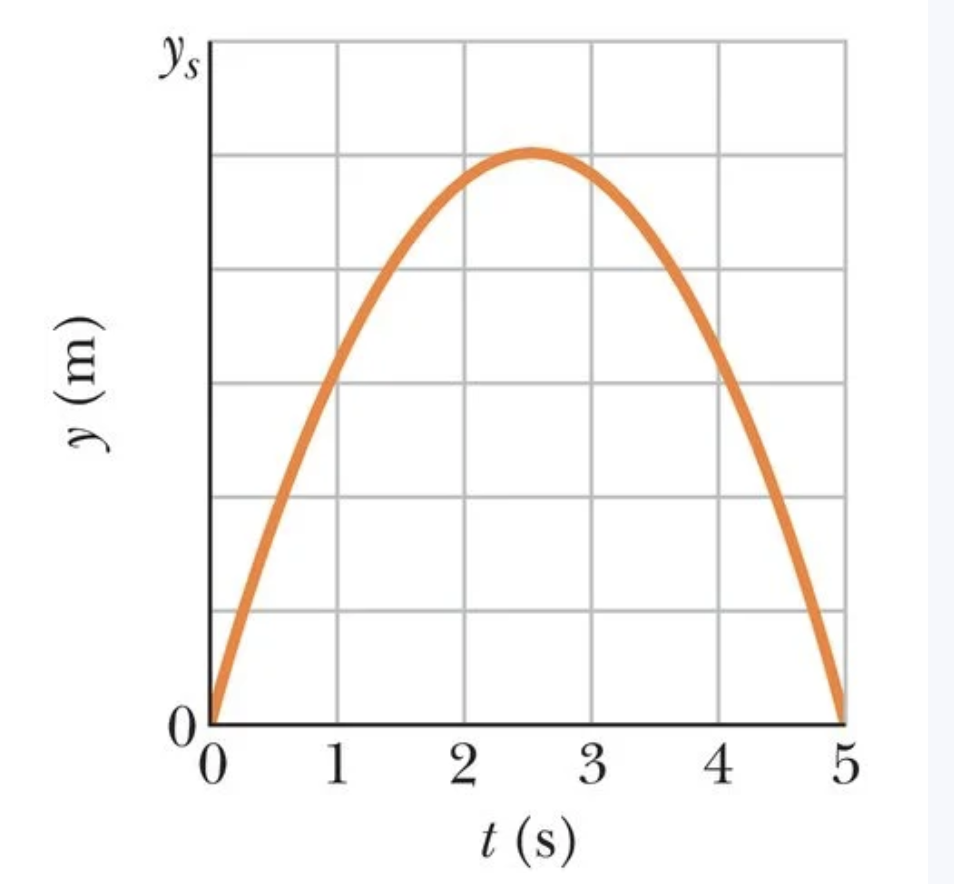
\includegraphics[scale=0.4]{2021-W1-Q4}
\end{figure}

\end{document}



%
%\begin{document}
%
%M&R Workshop 1 \\[3ex]
%
% 
%Your solution for \textcolor{red}{Question 3*} should be uploaded to Canvas.\\[1ex]
%
%
%
%% a) x= 12*(4^2) - 2*(4^3) = 64m
%% b) v = dx/dt =  24t - 6 t^2 = 24t*4- 6 *(4^2) = 0 m/s
%% c) a = dv/dt = 24 - 12t = 24 - 12*4 = - 24 m/s^2
%
%2. A rock is thrown vertically upward from ground level at time $t = 0$. At $t=1.5$ s it passes the top of a tall tower, and 1.0 s later it reaches its maximum height. What is the height of the tower?\\[3ex]
%
%% t1 = 2.5 s
%% a = -9.8 m/s^2
%% v = 0 
%% v = u +at => 0 = u + (-9.81)*(2.5) 0 = u + -24.5 so u = 24.5 m/s
%% s = ut + 0.5*a*t^2 = 24.5*1.5 + 0.5*-9.81*1.5*1.5 = 25.7 m
%
%\textcolor{red}{3*}. Two particles move along an x axis. The position of particle 1 is given by $x_1 = 6.00t^2 + 3.00t + 2.00$; the acceleration of particle 2 is given by $a_2 = -8.00t$ and, at $t = 0$, its velocity is  $v_2 = 20 ms^{-1}$. When the velocities of the particles match, what is their velocity?\\[3ex]
%
%% x_1 = 6 t^2 + 3t + 2
%% v_1 = 12t + 3
%% a_1 = 12
%% a2 = -8t 
%% u_2 = 20 
%% v = u +at =>  v_2 = 20 - 8t^2 
%% v1=v2 : 20 - 8t^2  = 12t + 3 => 8t^2 +12t  -17 = 0  at t=0.889
%% v1 = 12*0.889 +3 =13.7
%% v2 = 20 - 8*(0.889*0.889)  =13.7 correct.
%
%4.  A ball is shot vertically upward from the surface of another planet. A plot of y versus t for the ball is shown in the figure below, where $y$ is the height of the ball above its starting point and $t = 0$ at the instant the ball is shot. The figure?s vertical scaling is set by $y_s = 30.0$m. What are the magnitudes of :\\
%(a) the free-fall acceleration on the planet and \\[1ex]
%(b) the initial velocity of the ball?
%
%% t =5s
%% at y_s = 30.0, v=0 
%% it takes 2.5s to slow the ball to a stop from its uknown initial velocity u
%%  we know s, t, v , use s= 0.5* (u+v)t => 30 =0.5*u*2.5 so u= 30/(1.25)) = 24
%% v*v - u*u / 2s =a => - (24*24) / (2*30) = - 9.6

%\includegraphics[scale=0.3]{2021-W1-Q1}

 




 


